\documentclass[border=6pt]{standalone}
\usepackage{tikz}
\usetikzlibrary{arrows.meta,positioning,calc}
\begin{document}
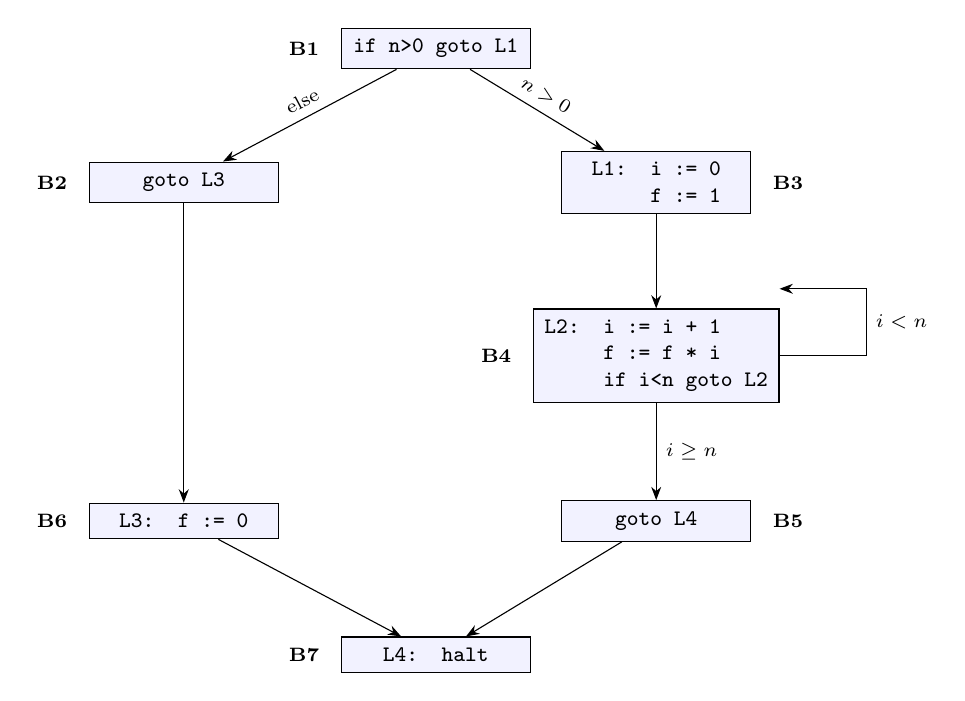
\begin{tikzpicture}[>=Stealth,font=\footnotesize,
 blk/.style={draw,align=left,inner sep=4pt,fill=blue!5,font=\ttfamily\footnotesize,minimum width=2.4cm},
 nm/.style={font=\scriptsize\bfseries}]
\node[blk] (b1) at (0,0) {if n>0 goto L1};
\node[blk] (b2) at (-3.2,-1.7) {goto L3};
\node[blk] (b3) at (2.8,-1.7) {L1: i := 0\\\phantom{L1: }f := 1};
\node[blk] (b4) at (2.8,-3.9) {L2: i := i + 1\\\phantom{L2: }f := f * i\\\phantom{L2: }if i<n goto L2};
\node[blk] (b5) at (2.8,-6.0) {goto L4};
\node[blk] (b6) at (-3.2,-6.0) {L3: f := 0};
\node[blk] (b7) at (0,-7.7) {L4: halt};
\node[nm,left=0.15cm of b1] {B1};
\node[nm,left=0.15cm of b2] {B2};
\node[nm,right=0.15cm of b3] {B3};
\node[nm,left=0.15cm of b4] {B4};
\node[nm,right=0.15cm of b5] {B5};
\node[nm,left=0.15cm of b6] {B6};
\node[nm,left=0.15cm of b7] {B7};
\draw[->] (b1) -- node[above,font=\scriptsize,sloped]{$n>0$} (b3);
\draw[->] (b1) -- node[above,font=\scriptsize,sloped]{else} (b2);
\draw[->] (b2) -- (b6);
\draw[->] (b3) -- (b4);
\draw[->] (b4) -- node[right,font=\scriptsize]{$i \ge n$} (b5);
\draw[->] (b4.east) -- ++(1.1,0) |- node[near start,right,font=\scriptsize]{$i<n$} ([yshift=0.25cm]b4.north east);
\draw[->] (b5) -- (b7);
\draw[->] (b6) -- (b7);
\end{tikzpicture}
\end{document}
